% !TeX spellcheck = en_US
\documentclass[a4paper]{scrartcl}

\usepackage[utf8]{inputenc}
\usepackage[english]{babel}
\usepackage[T1]{fontenc}
\usepackage{lmodern}
\usepackage{amsmath}
\usepackage{amssymb}
\usepackage{pdflscape}
\usepackage{geometry}
\usepackage{xcolor}
\usepackage{graphicx}
\usepackage{siunitx}
\usepackage{todonotes}
%\setlength{\parindent}{0pt}

\usepackage{biblatex}
\addbibresource{references.bib}


\geometry{a4paper, top=25mm, left=30mm, right=20mm, bottom=30mm,
headsep=10mm, footskip=12mm}

\newcommand{\itab}[1]{\hspace{0em}\rlap{#1}}
\newcommand{\tab}[1]{\hspace{.2\textwidth}\rlap{#1}}
\newcommand{\N}{\mathbb{N}}
\newcommand{\es}{\emptyset}

\title{Seminar on Algorithms for Compressed Graphs \\ Succinct Representation of Labeled Graphs}
\author{Matthias Dürksen}
\date{\today}
 

\begin{document}
\maketitle

\begin{abstract}
	Abstract...
\end{abstract}


\section{Introduction}\label{sec:introduction}

\subsection{Motivation}

\subsection{Fundamentals}

\subsection{Header}





\section{Succinct Representation}
The goal is to encode a graph as efficiently as possible and to be able to process query requests as efficiently as possible~\cite{SuccinctRepresentation}. Therefore triangulated planar graphs are converted into three trees, which in turn are converted into parenthesis. The parenthesis for the three trees are then converted to a nested parenthesis. This bracketed representation is the efficient coding where requests can be answered efficiently.





\subsection{Graph Model}
\todo{Änderung: Erst triangulated und anschließend als Erweiterung?}
A graph $G=(V,E)$ consists of a set of nodes $V$ and a set of edges $E$. We consider undirected graphs so that the set of edges $E$ is undirected.
The succint representation is constructed so that the coding only works for a subset of graphs, the undirected planar graph. A planar graph is a $G$ graph that can represent nodes in a two dimensional plane so that no edges intersect with another edge. For an example of a planar graph, see Figure~\ref{fig:planar}.


\begin{figure}[h]
	\centering
	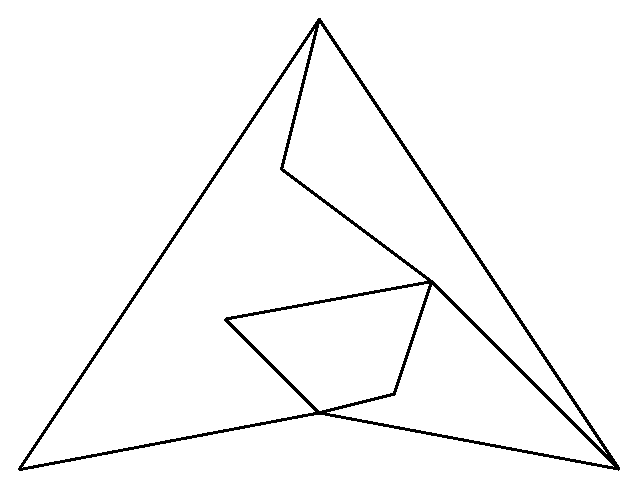
\includegraphics[width=0.4\textwidth]{img/planar}
	\caption{A planar graph}
	\label{fig:planar}
\end{figure}


In the first step, the planar graphs are converted to a triangulated planar graph.
\todo{Explain how}
The graph from Figure~\ref{fig:planar} becomes a triangulated planar graph by the graph, see Figure~\ref{fig:triangulated}.
\todo{Why always three vertices}
Therefore it can be assumed that the graph always has three vertices which are adjacent to each other. These edges form the convex envelope of the graph, where we call the three nodes $v_0,v_1$ and $v_{n-1}$.



\begin{figure}[h]
	\centering
	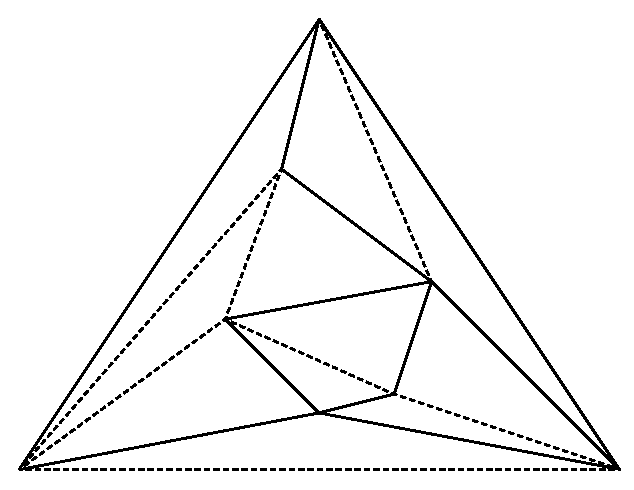
\includegraphics[width=0.4\textwidth]{img/triangulated}
	\caption{The triangulated  graph from Figure~\ref{fig:planar}}
	\label{fig:triangulated}
\end{figure}
\todo{Explain complexity for space/time}

\subsection{Schnyder realizer}
The graph is divided into three trees for further compression. For this a Schnyder realizer~\cite{schnyder} is used. This divides the graph into three trees $T_0,T_1,T_2$. Each inner edge is assigned to one of the three trees. These are assigned so that each inner node has three outgoing edges, where each outgoing edge contains a different tree. \todo{Explain: Why directed} In addition, the node can have incoming edges, where these must be arranged in a certain way. In Figure~\ref{fig:schnyderRealizer} we see the arrangement. The edges are arranged according to the pattern outgoing $T_0$, incoming $T_1$, outgoing $T_2$, incoming $T_0$, outgoing $T_1$, incoming $T_2$. The trees $T_0,T_1,T_2$ have as root the node $v_0,v_1,v_{n-1}$.
Thus the graph, see Figure~\ref{fig:example}, is divided into three trees, see Figure~\ref{exampleSchnyder}.\todo{Vlt explain in more detail how the construction is made}.
\begin{figure}[h]
	\centering
	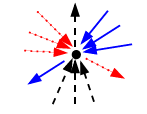
\includegraphics[width=0.7\textwidth]{img/schnyderRealizer}
	\caption{Structure of the edges for an internal node in the graph. }
	\label{fig:schnyderrealizer}
\end{figure}



\begin{figure}[h]
	\centering
	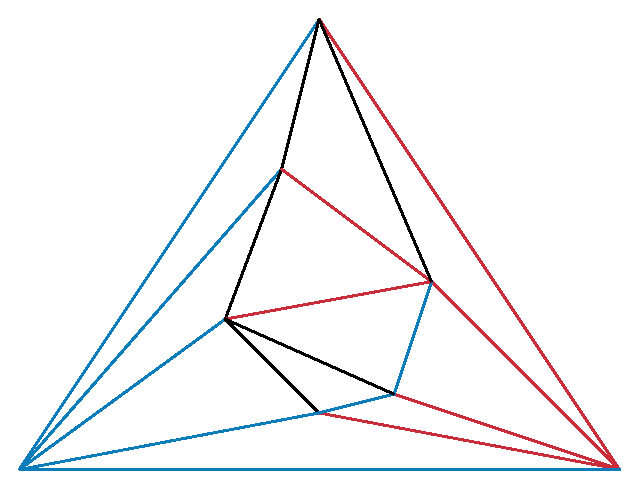
\includegraphics[width=0.6\textwidth]{img/exampleSchnyder}
	\caption{The trees in the graph which are formed on the basis of the Schnyder realizer}
	\label{fig:exampleSchnyder}
\end{figure}
\todo{Change to directed edges}


\subsection{Traversal Orders}
The graph is divided into three subtrees using a Schnyder realizer, but the edges lying on the convex hull of the graph are not yet contained in the trees. In addition we have to number the nodes for the following brackets. \todo{why are the other traversal orders needed}
The two edges $(v_1,v_0),(v_{n-1},v_0)$, which lie on the convex hull, are assigned to the tree $T_0$ and the edge $(v_{n-1},v_1)$ is assigned to the tree $T_1$. So $T_0$ is an canonical spanning tree.

To number the nodes in $T_0$ a depth search in the node $v_0$ is executed counterclockwise and the visiting nodes are numbered ascending, see Figure~\ref{fig:exampleTraversal}.

\begin{figure}[h]
	\centering
	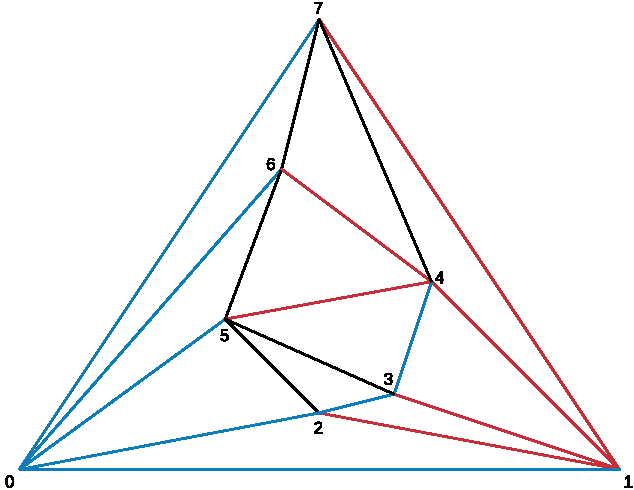
\includegraphics[width=0.6\textwidth]{img/exampleTraversal}
	\caption{The partitioned graph with the numbering by $T_0$}
	\label{fig:exampleTraversal}
\end{figure}




\subsection{Parenthesis}
The aim is to combine the trees with the help of brackets to a common brackets representation. To do this, we first generate the parenthesis for the individual trees and then combine them. For each of the trees $T_0,T_1,T_2$ the parenthesis is generated differently. We designate a pair of parenthesis as an opening parenthesis followed by a closing parenthesis.

Let's first look at the parenthesis for the tree $T_0$. Starting from the root $v_0$ this parenthesis is created. To encode the root we use pairs of brackets. For each of the children of depth 1 we create another pair of brackets in the pair of brackets. If a child $a$ of depth 1 has children of its own, its children are displayed as a pair of parenthesis in the pair of parenthesis for the node $a$. The children are included in the parenthesis on a level countering the clockwise direction. Thus the following recursive definition follows:

For all nodes $v$ of depth i applies:



\begin{equation}
 i&=0 \rightarrow \text{pair of parenthesis}\\
 
i&>0 \rightarrow \text{insert pair of parenthesis in } parent(v)
\end{equation}
\todo{Geordnet}

Figure~\ref{fig:parenthesisOne} zeigt wie eine solche Klammerdarstellung für den Baum $T_0$ anhand unseres Beispiel aussieht.

\begin{figure}[h]
	\centering
	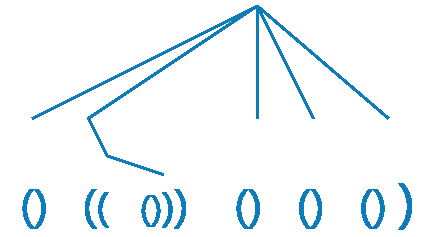
\includegraphics[width=0.7\textwidth]{img/parenthesisOne}
	\caption{The parenthesis of the  tree $T_0$}
	\label{fig:parenthesisOne}
\end{figure}





For the tree $T_1$ the parenthesis representation is generated differently. A pair of parenthesis is created for each child of the root $v_1$, but the pairs of parenthesis are not written one after the other on the same level, but nested together. Here the edges are passed counterclockwise again, so that the child $a$, which is visited first, is on the outside and the other children are written into the brace pair of $a$. If a node has $v$ children, the children are also nested into each other and packed in the place of the parenthesis, which comes directly after the closing parenthesis of $a$.\todo{example}. The parenthesis for the tree $T_1$ from our example is shown in Figure~\ref{fig:parenthesisTwo}.


\begin{figure}[h]
	\centering
	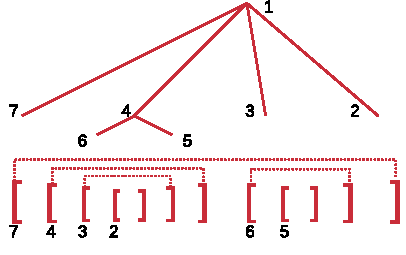
\includegraphics[width=0.7\textwidth]{img/parenthesisTwo}
	\caption{The parenthesis of the  tree $T_1$}
	\label{fig:parenthesisTwo}
\end{figure}


The parenthesis for the tree $T_2$ is created similar to the parenthesis for $T_1$. Again the children are nested again, but the children are passed clockwise. If a node has $v$ children, these nested children are now written in front of the opening parenthesis of $v$. This procedure is illustrated by the example in Figure~\ref{fig:parenthesisTrees}c).\todo{add graphic}




The three parenthesis must now be combined so that no information about the graph is lost. The parenthesis of a tree $T_i$ is called $S_i$. In order to be able to distinguish the parts of the different parenthesis according to the combination, we use different parenthesis symbols for each parenthesis. The parenthesis $S_0$ serves as the basic structure. The other two parenthesis are included in this. The parenthesis are created as follows.

\begin{itemize}
	\item $\forall e=(v_i,v_j)\in T_1: \text{ insert } '[' \text{ before } parenthesis(v_i)\in S_0 \text{ closed.}$
	\item $\forall e=(v_i,v_j)\in T_1: \text{ insert } ']' \text{ after } parenthesis(v_i)\in S_0 \text{ opened.}$
	\item $\forall e=(v_i,v_j)\in T_2: \text{ insert } ']' \text{ after } parenthesis(v_i)\in S_0 \text{ opened.}$
	\item $\forall e=(v_i,v_j)\in T_2: \text{ insert } '[' \text{ before } parenthesis(v_i)\in S_0 \text{ closed.}$
\end{itemize}
In the example, the three parenthesis become the combined representation in Figure~\ref{fig:parenthesisCombi}.
This creates a parenthesis that contains three types of parenthesis, each parenthesis still being a valid parenthesis.

\begin{figure}[h]
	\centering
	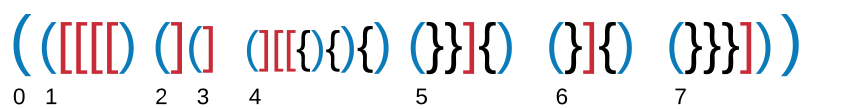
\includegraphics[width=0.8\textwidth]{img/parenthesisCombi}
	\caption{The parenthesis of the merges trees}
	\label{fig:parenthesisCombi}
\end{figure}

\subsection{Querys}

\subsection{Size complexity}

\todo{Modify later, propaly not completly correct}
The parenthesis representation consists of three different types of parenthesis, whereby 2 symbols are required for each type (opening and closing parenthesis). This means that a total of 6 different characters are required. Each edge of the graph is coded exactly once and one opening and one closing bracket are required per edge. Nodes do not have to be encoded separately, since the information indirectly contains the edges. Thus $2m$ symbols are needed for the representation, at m the number of edges is in G.


\subsection{Reconstruction of the graph}

\section{Extensions}

node/edge labels\\\\
k-page Graphs


\section{Conclusion \& Future Work}



\pagebreak


\printbibliography







\end{document}